\hypertarget{Builder__graphs_8h}{
\section{include/Builders/Builder\_\-graphs.h File Reference}
\label{Builder__graphs_8h}\index{include/Builders/Builder\_\-graphs.h@{include/Builders/Builder\_\-graphs.h}}
}
Header with the functions for build all kind of graphs for the attribute grammar.  


{\tt \#include $<$map$>$}\par
{\tt \#include $<$string$>$}\par
{\tt \#include $<$vector$>$}\par
{\tt \#include $<$boost/graph/adjacency\_\-list.hpp$>$}\par
{\tt \#include \char`\"{}../Attr\_\-grammar/Attr\_\-grammar.h\char`\"{}}\par
{\tt \#include \char`\"{}../Expression\_\-tree/Expr\_\-leaf.h\char`\"{}}\par


Include dependency graph for Builder\_\-graphs.h:\nopagebreak
\begin{figure}[H]
\begin{center}
\leavevmode
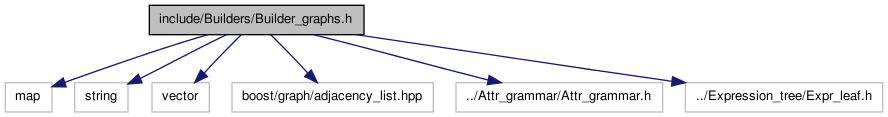
\includegraphics[width=356pt]{Builder__graphs_8h__incl}
\end{center}
\end{figure}


This graph shows which files directly or indirectly include this file:\nopagebreak
\begin{figure}[H]
\begin{center}
\leavevmode
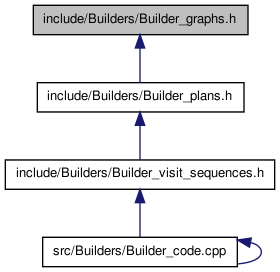
\includegraphics[width=420pt]{Builder__graphs_8h__dep__incl}
\end{center}
\end{figure}
\subsection*{Classes}
\begin{CompactItemize}
\item 
struct \hyperlink{structgenevalmag_1_1vertex__data__t}{genevalmag::vertex\_\-data\_\-t}
\item 
class \hyperlink{classgenevalmag_1_1Builder__graphs}{genevalmag::Builder\_\-graphs}
\end{CompactItemize}
\subsection*{Namespaces}
\begin{CompactItemize}
\item 
namespace \hyperlink{namespacegenevalmag}{genevalmag}
\end{CompactItemize}
\subsection*{Typedefs}
\begin{CompactItemize}
\item 
typedef adjacency\_\-list$<$ hash\_\-setS, vecS, directedS, property\_\-vertex\_\-dp $>$ \hyperlink{namespacegenevalmag_4a96de9ebfc7d48233406ab9cad55cb5}{genevalmag::Graph}
\item 
typedef Graph::vertex\_\-descriptor \hyperlink{namespacegenevalmag_2aae7b018fc2a9afae131bbf639181b5}{genevalmag::Vertex}
\end{CompactItemize}
\subsection*{Variables}
\begin{CompactItemize}
\item 
typedef$<$ vertex\_\-data\_\-t, constgenevalmag::Expr\_\-leaf $\ast$ $>$ \hyperlink{namespacegenevalmag_17d2e2ff96dab5c47f9d82e32317997c}{genevalmag::property\_\-vertex\_\-dp}
\end{CompactItemize}


\subsection{Detailed Description}
Header with the functions for build all kind of graphs for the attribute grammar. 

\begin{Desc}
\item[Date:]17/02/2010 \end{Desc}
\begin{Desc}
\item[Author:]Kilmurray, Gerardo Luis $<$\href{mailto:gerakilmurray@gmail.com}{\tt gerakilmurray@gmail.com}$>$ 

Picco, Gonzalo Martín $<$\href{mailto:gonzalopicco@gmail.com}{\tt gonzalopicco@gmail.com}$>$ \end{Desc}


Definition in file \hyperlink{Builder__graphs_8h-source}{Builder\_\-graphs.h}.
